\chapter{Pretest and posttest statistics}
\label{app:learning_gain}

\section{Descriptives of the knowledge questions}

\begin{longtable}[c]{@{}lrrrrrrrrrr@{}}
\caption{Flashcard condition}\\
\endfirsthead
\endhead
\toprule\addlinespace
& N & min & max & mean & var & skew & kurt & norm-t &
norm-p & $\alpha$
\\
\addlinespace
\midrule
\textbf{ctt:total} & 24 & 0 & 6 & 1.29 & 4.13 & 1.34 & 0.40 & 8.732 &
0.0127 & 0.6958
\\\addlinespace
\textbf{ctt:pretest} & 12 & 0 & 3 & 0.67 & 1.15 & 1.16 & -0.19 & 4.546 &
0.1030 & 0.4290
\\\addlinespace
\textbf{ctt:posttest} & 12 & 0 & 6 & 1.92 & 6.63 & 0.70 & -1.29 & 3.371
& 0.1854 & 0.7261
\\\addlinespace
\textbf{ctt:abs\_learn\_gain} & 12 & -3 & 6 & 1.25 & 8.39 & 0.47 & -0.84
& 0.900 & 0.6378 & 0.4290
\\\addlinespace
\textbf{ctt:rel\_learn\_gain} & 12 & 0 & 0 & 0.04 & 0.00 & 0.43 & -0.86
& 0.810 & 0.6671 & 0.4290
\\\addlinespace
\textbf{irt:total} & 24 & -1 & 4 & -0.03 & 3.05 & 1.05 & 0.04 & 5.537 &
0.0627 & 0.4556
\\\addlinespace
\textbf{irt:pretest} & 12 & 0 & 0 & 0.00 & 0.08 & 0.62 & 0.07 & 2.059 &
0.3573 & 0.0687
\\\addlinespace
\textbf{irt:posttest} & 12 & -2 & 3 & -0.01 & 2.70 & 0.61 & 0.63 & 3.146
& 0.2074 & 0.3769
\\\addlinespace
\textbf{irt:abs\_learn\_gain} & 12 & -2 & 3 & -0.01 & 2.87 & 0.91 & 0.61
& 4.553 & 0.1026 & 0.0687
\\\addlinespace
\textbf{irt:rel\_learn\_gain} & 12 & 0 & 0 & 0.02 & 0.00 & 0.90 & 0.59 &
4.487 & 0.1061 & 0.0687
\\\addlinespace
\textbf{fixed irt:total} & 24 & -4 & 3 & -0.83 & 4.14 & 0.58 & -0.36
& 1.812 & 0.4042 & 0.5294
\\\addlinespace
\textbf{fixed irt:pretest} & 12 & 1 & 3 & 2.60 & 0.17 & 0.43 & 0.39 &
2.010 & 0.3661 & 0.1088
\\\addlinespace
\textbf{fixed irt:posttest} & 12 & -2 & 3 & -0.07 & 2.71 & 0.61 &
0.63 & 3.188 & 0.2031 & 0.3774
\\\addlinespace
\textbf{fixed irt:abs\_learn\_gain} & 12 & -4 & 1 & -2.67 & 2.91 &
1.01 & 0.64 & 5.199 & 0.0743 & 0.1088
\\\addlinespace
\textbf{fixed irt:rel\_learn\_gain} & 12 & 0 & 0 & -0.03 & 0.00 &
1.01 & 0.62 & 5.132 & 0.0769 & 0.1088
\\\addlinespace
\bottomrule
    \label{tab:know_fc}
\end{longtable}

\begin{figure}
    \centering
    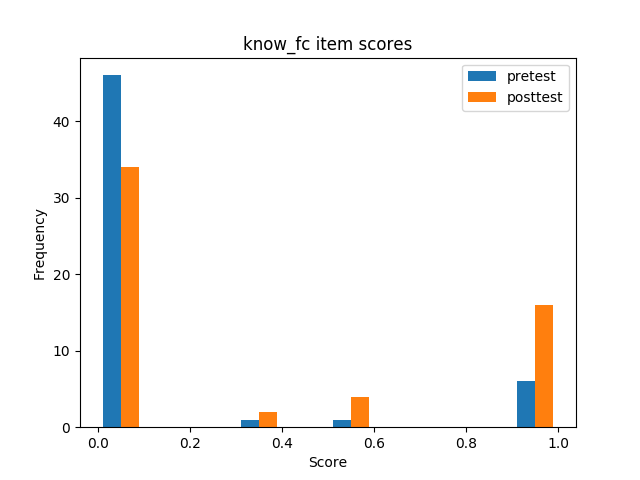
\includegraphics[width=.7\textwidth]{img/know_fc_diff.png}
    \caption{A histogram depicting the scores on the knowledge section of the pre- and posttest per item by flashcard users}
    \label{fig:know_fc_diff}
\end{figure}
\begin{figure}
    \centering
    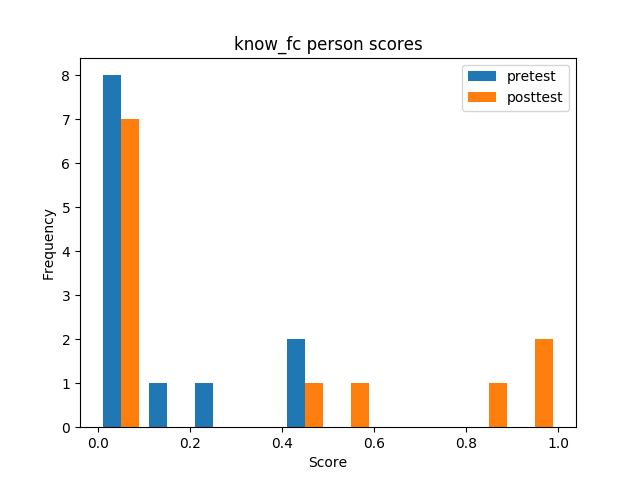
\includegraphics[width=.7\textwidth]{img/know_fc_abil.png}
    \caption{A histogram depicting the scores on the knowledge section of the pre- and posttest per flashcard user}
    \label{fig:know_fc_abil}
\end{figure}

\begin{longtable}[c]{@{}lrrrrrrrrrr@{}}
\caption{Flashmap condition}
\endfirsthead
\endhead
\toprule\addlinespace
& N & min & max & mean & var & skew & kurt & norm-t &
norm-p & $\alpha$
\\\addlinespace
\midrule
\textbf{ctt:total} & 22 & 0 & 7 & 1.32 & 4.89 & 1.48 & 0.77 & 10.348 &
0.0057 & 0.7424
\\\addlinespace
\textbf{ctt:pretest} & 11 & 0 & 1 & 0.18 & 0.16 & 1.65 & 0.72 & 9.711 &
0.0078 & -0.1132
\\\addlinespace
\textbf{ctt:posttest} & 11 & 0 & 7 & 2.45 & 7.27 & 0.45 & -1.31 & 2.304
& 0.3160 & 0.6841
\\\addlinespace
\textbf{ctt:abs\_learn\_gain} & 11 & -1 & 7 & 2.27 & 7.42 & 0.45 & -1.14
& 1.448 & 0.4848 & -0.1132
\\\addlinespace
\textbf{ctt:rel\_learn\_gain} & 11 & 0 & 0 & 0.05 & 0.00 & 0.44 & -1.15
& 1.490 & 0.4747 & -0.1132
\\\addlinespace
\textbf{irt:total} & 22 & -2 & 4 & -0.03 & 3.02 & 0.62 & 0.46 & 3.124 &
0.2097 & 0.3942
\\\addlinespace
\textbf{irt:pretest} & 11 & 0 & 0 & -0.00 & 0.00 & 1.65 & 0.72 & 9.711 &
0.0078 & 0.0000
\\\addlinespace
\textbf{irt:posttest} & 11 & -1 & 1 & -0.00 & 0.76 & -0.00 & 2.50 &
6.534 & 0.0381 & 0.1362
\\\addlinespace
\textbf{irt:abs\_learn\_gain} & 11 & -1 & 1 & -0.00 & 0.76 & -0.00 &
2.50 & 6.534 & 0.0381 & 0.0000
\\\addlinespace
\textbf{irt:rel\_learn\_gain} & 11 & 0 & 0 & 0.02 & 0.00 & 0.00 & 2.50 &
7.592 & 0.0225 & 0.0000
\\\addlinespace
\textbf{fixed irt:total} & 22 & -4 & 3 & -0.80 & 3.94 & 0.17 & 0.04 &
0.556 & 0.7575 & 0.4530
\\\addlinespace
\textbf{fixed irt:pretest} & 11 & 0 & 0 & 0.11 & 0.00 & 0.00 & -3.00
& 1.057 & 0.5894 & 0.0000
\\\addlinespace
\textbf{fixed irt:posttest} & 11 & 2 & 4 & 3.27 & 0.15 & -0.02 & 2.44
& 6.403 & 0.0407 & 0.1020
\\\addlinespace
\textbf{fixed irt:abs\_learn\_gain} & 11 & 2 & 4 & 3.17 & 0.15 &
-0.02 & 2.44 & 6.403 & 0.0407 & 0.0000
\\\addlinespace
\textbf{fixed irt:rel\_learn\_gain} & 11 & 0 & 0 & 0.07 & 0.00 &
-0.02 & 2.44 & 6.403 & 0.0407 & 0.0000
\\\addlinespace
\bottomrule
    \label{tab:know_fm}
\end{longtable}

\begin{figure}
    \centering
    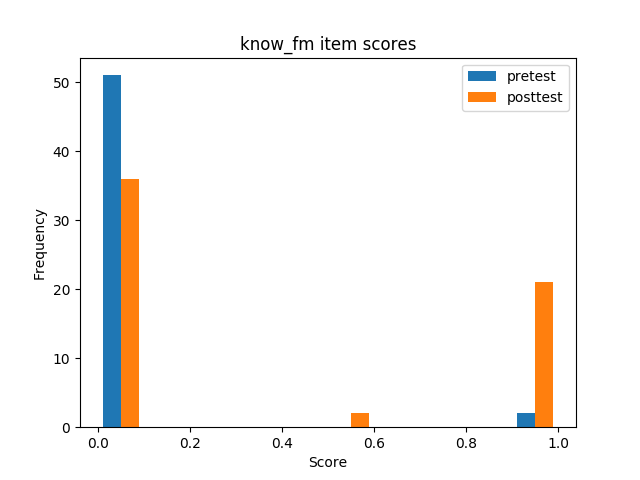
\includegraphics[width=.7\textwidth]{img/know_fm_diff.png}
    \caption{A histogram depicting the scores on the knowledge section of the pre- and posttest per item by flashmap users}
    \label{fig:know_fm_diff}
\end{figure}
\begin{figure}
    \centering
    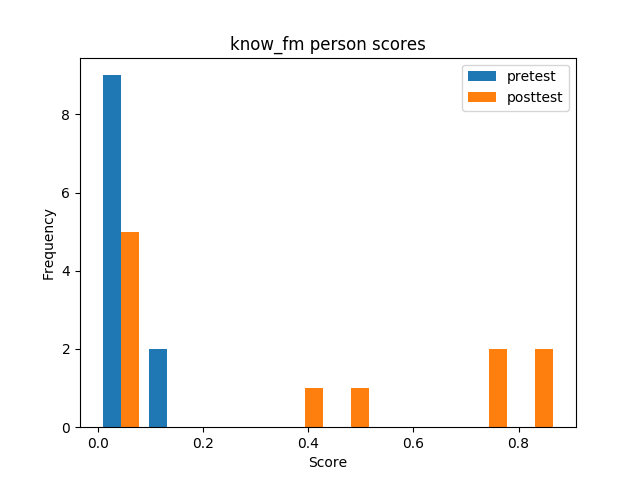
\includegraphics[width=.7\textwidth]{img/know_fm_abil.png}
    \caption{A histogram depicting the scores on the knowledge section of the pre- and posttest per flashmap user}
    \label{fig:know_fm_abil}
\end{figure}

\begin{longtable}[c]{@{}lrrrrrrrrrr@{}}
\caption{Combined conditions}
\endfirsthead
\endhead
\toprule\addlinespace
& N & min & max & mean & var & skew & kurt & norm-t &
norm-p & $\alpha$
\\\addlinespace
\midrule
\textbf{ctt:total} & 46 & 0 & 7 & 1.30 & 4.39 & 1.42 & 0.64 & 14.471 &
0.0007 & 0.7112
\\\addlinespace
\textbf{ctt:pretest} & 23 & 0 & 3 & 0.43 & 0.71 & 1.83 & 2.28 & 17.317 &
0.0002 & 0.3937
\\\addlinespace
\textbf{ctt:posttest} & 23 & 0 & 7 & 2.17 & 6.70 & 0.58 & -1.30 & 6.839
& 0.0327 & 0.6851
\\\addlinespace
\textbf{ctt:abs\_learn\_gain} & 23 & -3 & 7 & 1.74 & 7.84 & 0.40 & -0.93
& 2.023 & 0.3637 & 0.3937
\\\addlinespace
\textbf{ctt:rel\_learn\_gain} & 23 & 0 & 0 & 0.03 & 0.00 & 0.39 & -0.93
& 1.977 & 0.3722 & 0.3937
\\\addlinespace
\textbf{irt:total} & 46 & -3 & 5 & -0.10 & 4.92 & 0.98 & -0.23 & 7.303 &
0.0259 & 0.5856
\\\addlinespace
\textbf{irt:pretest} & 23 & -2 & 2 & -0.00 & 1.22 & 0.97 & 2.19 & 9.614
& 0.0082 & 0.2141
\\\addlinespace
\textbf{irt:posttest} & 23 & -3 & 3 & -0.02 & 3.68 & 0.87 & -0.19 &
3.757 & 0.1528 & 0.4740
\\\addlinespace
\textbf{irt:abs\_learn\_gain} & 23 & -4 & 4 & -0.02 & 5.31 & 0.42 &
-0.29 & 0.967 & 0.6166 & 0.2141
\\\addlinespace
\textbf{irt:rel\_learn\_gain} & 23 & 0 & 0 & 0.01 & 0.00 & 0.38 & -0.27
& 0.833 & 0.6592 & 0.2141
\\\addlinespace
\textbf{fixed irt:total} & 46 & -5 & 3 & -1.85 & 5.68 & 0.80 & -0.29
& 5.224 & 0.0734 & 0.6710
\\\addlinespace
\textbf{fixed irt:pretest} & 23 & -2 & 2 & -0.01 & 1.22 & 0.98 & 2.19
& 9.677 & 0.0079 & 0.2142
\\\addlinespace
\textbf{fixed irt:posttest} & 23 & -4 & 3 & -0.88 & 5.74 & 0.31 &
-0.53 & 0.564 & 0.7541 & 0.5859
\\\addlinespace
\textbf{fixed irt:abs\_learn\_gain} & 23 & -7 & 4 & -0.88 & 8.23 &
-0.21 & 0.11 & 0.742 & 0.6900 & 0.2142
\\\addlinespace
\textbf{fixed irt:rel\_learn\_gain} & 23 & 0 & 0 & 0.00 & 0.00 &
-0.26 & 0.19 & 1.015 & 0.6019 & 0.2142
\\\addlinespace
\bottomrule
    \label{tab:know_gen}
\end{longtable}

\begin{figure}
    \centering
    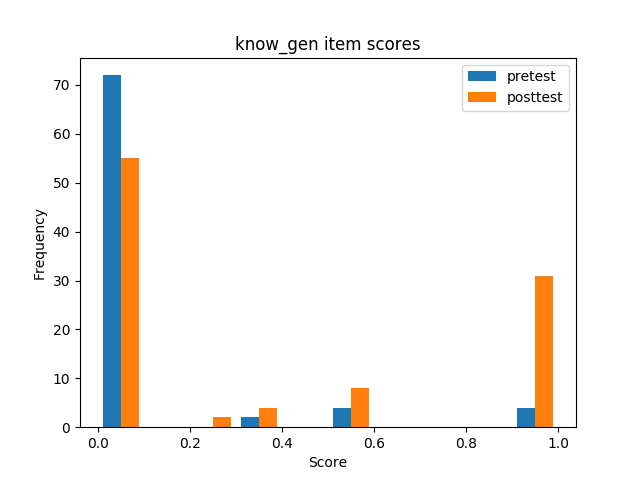
\includegraphics[width=.7\textwidth]{img/know_gen_diff.png}
    \caption{A histogram depicting the scores on the knowledge section of the pre- and posttest per item}
    \label{fig:know_gen_diff}
\end{figure}
\begin{figure}
    \centering
    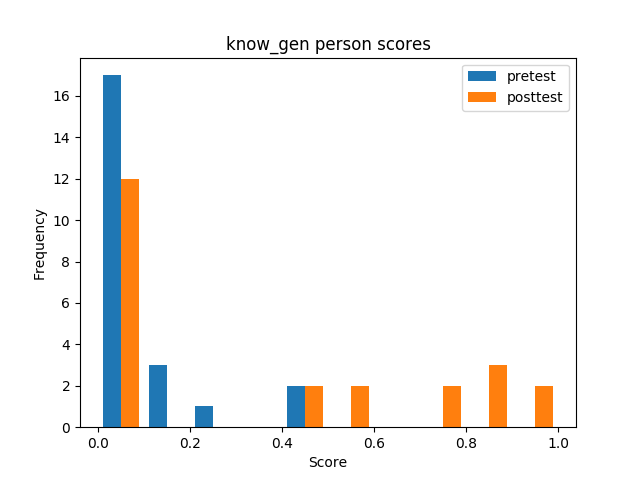
\includegraphics[width=.7\textwidth]{img/know_gen_abil.png}
    \caption{A histogram depicting the scores on the knowledge section of the pre- and posttest per user}
    \label{fig:know_gen_abil}
\end{figure}

\FloatBarrier
\section{Comparisons of the knowledge questions}

\FloatBarrier
\subsection{Pre- and posttest comparisons}

\begin{longtable}[c]{@{}lrrrr@{}}
\caption{Flashcard condition}
\endfirsthead
\endhead
\toprule\addlinespace
& \textbf{MW k} & \textbf{MW p} &
\textbf{t-test k} & \textbf{t-test p}
\\\addlinespace
\midrule
\textbf{ctt} & -1.552 & 0.1348 & -1.552 & 0.1418
\\\addlinespace
\textbf{irt} & 0.016 & 0.9872 & 0.016 & 0.9873
\\\addlinespace
\textbf{fixed irt} & 5.454 & 0.0000 & 5.454 & 0.0001
\\\addlinespace
\bottomrule
    \label{tab:know_pp_fc_comp}
\end{longtable}

\begin{longtable}[c]{@{}lrrrr@{}}
\caption{Flashmap condition}
\endfirsthead
\endhead
\toprule\addlinespace
& \textbf{MW k} & \textbf{MW p} &
\textbf{t-test k} & \textbf{t-test p}
\\\addlinespace
\midrule
\textbf{ctt} & -2.764 & 0.0120 & -2.764 & 0.0192
\\\addlinespace
\textbf{irt} & -0.000 & 1.0000 & -0.000 & 1.0000
\\\addlinespace
\textbf{fixed irt} & -27.206 & 0.0000 & -27.206 & 0.0000
\\\addlinespace
\bottomrule
    \label{tab:know_pp_fm_comp}
\end{longtable}

\begin{longtable}[c]{@{}lrrrr@{}}
\caption{Combined conditions}
\endfirsthead
\endhead
\toprule\addlinespace
& \textbf{MW k} & \textbf{MW p} &
\textbf{t-test k} & \textbf{t-test p}
\\\addlinespace
\midrule
\textbf{ctt} & -3.065 & 0.0037 & -3.065 & 0.0049
\\\addlinespace
\textbf{irt} & 0.051 & 0.9597 & 0.051 & 0.9598
\\\addlinespace
\textbf{fixed irt} & 1.591 & 0.1187 & 1.591 & 0.1217
\\\addlinespace
\bottomrule
    \label{tab:know_pp_gen_comp}
\end{longtable}

\FloatBarrier
\subsection{Learning gain comparisons between conditions}

\begin{longtable}[c]{@{}lrrrr@{}}
\caption{Classical test theory}
\endfirsthead
\endhead
\toprule\addlinespace
& \textbf{MW k} & \textbf{MW p} &
\textbf{t-test k} & \textbf{t-test p}
\\\addlinespace
\midrule
\textbf{total} & -0.042 & 0.9664 & -0.042 & 0.9665
\\\addlinespace
\textbf{pretest} & 1.407 & 0.1739 & 1.456 & 0.1669
\\\addlinespace
\textbf{posttest} & -0.489 & 0.6297 & -0.488 & 0.6305
\\\addlinespace
\textbf{abs\_learn\_gain} & -0.870 & 0.3940 & -0.873 & 0.3927
\\\addlinespace
\textbf{rel\_learn\_gain} & -0.747 & 0.4635 & -0.751 & 0.4611
\\\addlinespace
\bottomrule
    \label{tab:know_cond_ctt_comp}
\end{longtable}

\begin{longtable}[c]{@{}lrrrr@{}}
\caption{Item response theory}
\endfirsthead
\endhead
\toprule\addlinespace
& \textbf{MW k} & \textbf{MW p} &
\textbf{t-test k} & \textbf{t-test p}
\\\addlinespace
\midrule
\textbf{total} & -0.001 & 0.9989 & -0.001 & 0.9989
\\\addlinespace
\textbf{pretest} & 0.000 & 1.0000 & 0.000 & 1.0000
\\\addlinespace
\textbf{posttest} & -0.014 & 0.9889 & -0.014 & 0.9887
\\\addlinespace
\textbf{abs\_learn\_gain} & -0.014 & 0.9892 & -0.014 & 0.9889
\\\addlinespace
\textbf{rel\_learn\_gain} & 0.072 & 0.9436 & 0.074 & 0.9423
\\\addlinespace
\bottomrule
    \label{tab:know_cond_irt_comp}
\end{longtable}

\begin{longtable}[c]{@{}lrrrr@{}}
\caption{Item response theory with fixed item difficulties}
\endfirsthead
\endhead
\toprule\addlinespace
& \textbf{MW k} & \textbf{MW p} &
\textbf{t-test k} & \textbf{t-test p}
\\\addlinespace
\midrule
\textbf{total} & -0.050 & 0.9602 & -0.050 & 0.9602
\\\addlinespace
\textbf{pretest} & 20.261 & 0.0000 & 21.204 & 0.0000
\\\addlinespace
\textbf{posttest} & -6.549 & 0.0000 & -6.821 & 0.0000
\\\addlinespace
\textbf{abs\_learn\_gain} & -11.067 & 0.0000 & -11.531 & 0.0000
\\\addlinespace
\textbf{rel\_learn\_gain} & -10.401 & 0.0000 & -10.845 & 0.0000
\\\addlinespace
\bottomrule
    \label{tab:know_cond_adj_irt_comp}
\end{longtable}

\begin{figure}
    \centering
    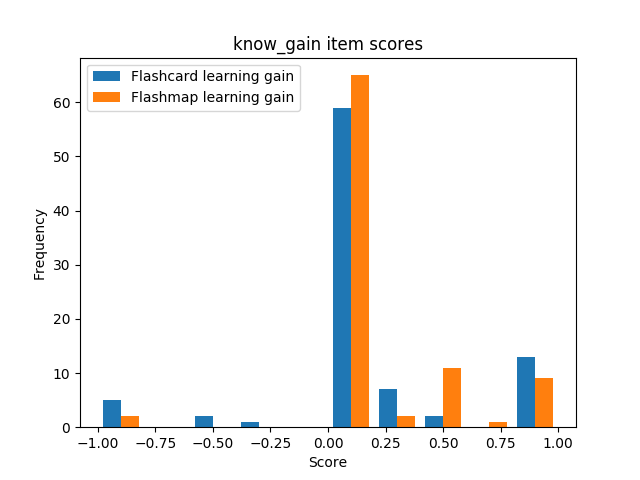
\includegraphics[width=.7\textwidth]{img/know_gain_diff.png}
    \caption{A comparison of figure~\protect\ref{fig:know_fc_diff} and~\protect\ref{fig:know_fm_diff}, with the pretest score subtracted from the posttest score}
    \label{fig:know_gain_diff}
\end{figure}

\FloatBarrier
\section{Descriptives of the comprehension questions}

\begin{longtable}[c]{@{}lrrrrrrrrrr@{}}
\caption{Flashcard condition}
\endfirsthead
\endhead
\toprule\addlinespace
& N & min & max & mean & var & skew & kurt & norm-t &
norm-p & $\alpha$
\\\addlinespace
\midrule
\textbf{ctt:total} & 24 & 0 & 6 & 1.33 & 4.23 & 1.19 & -0.05 & 6.646 &
0.0361 & 0.7215
\\\addlinespace
\textbf{ctt:pretest} & 12 & 0 & 4 & 0.33 & 1.33 & 3.02 & 7.09 & 33.648 &
0.0000 & 0.7670
\\\addlinespace
\textbf{ctt:posttest} & 12 & 0 & 6 & 2.33 & 5.33 & 0.41 & -1.25 & 2.077
& 0.3540 & 0.6450
\\\addlinespace
\textbf{ctt:abs\_learn\_gain} & 12 & 0 & 6 & 2.00 & 5.45 & 0.72 & -0.96
& 2.091 & 0.3516 & 0.6450
\\\addlinespace
\textbf{ctt:rel\_learn\_gain} & 12 & 0 & 0 & 0.07 & 0.00 & 0.72 & -0.95
& 2.097 & 0.3504 & 0.6450
\\\addlinespace
\textbf{irt:total} & 24 & -2 & 4 & 0.05 & 4.71 & 0.80 & -0.83 & 4.030 &
0.1333 & 0.6583
\\\addlinespace
\textbf{irt:pretest} & 12 & -1 & 4 & -0.09 & 2.62 & 2.47 & 5.19 & 26.077
& 0.0000 & 0.3406
\\\addlinespace
\textbf{irt:posttest} & 12 & -2 & 2 & 0.01 & 3.51 & 0.00 & -1.31 & 1.869
& 0.3929 & 0.7510
\\\addlinespace
\textbf{irt:abs\_learn\_gain} & 12 & -3 & 3 & 0.10 & 5.54 & -0.07 &
-1.19 & 1.211 & 0.5459 & 0.3406
\\\addlinespace
\textbf{irt:rel\_learn\_gain} & 12 & 0 & 0 & 0.02 & 0.00 & -0.15 & -1.11
& 0.886 & 0.6420 & 0.3406
\\\addlinespace
\textbf{fixed irt:total} & 24 & -3 & 3 & -1.15 & 3.83 & 0.90 & -0.52
& 4.058 & 0.1315 & 0.6673
\\\addlinespace
\textbf{fixed irt:pretest} & 12 & 0 & 5 & 0.42 & 2.58 & 2.72 & 6.04 &
29.551 & 0.0000 & 0.3207
\\\addlinespace
\textbf{fixed irt:posttest} & 12 & -3 & 1 & -0.87 & 3.16 & 0.03 &
-1.30 & 1.835 & 0.3994 & 0.7480
\\\addlinespace
\textbf{fixed irt:abs\_learn\_gain} & 12 & -5 & 2 & -1.28 & 5.01 &
-0.15 & -1.04 & 0.652 & 0.7218 & 0.3207
\\\addlinespace
\textbf{fixed irt:rel\_learn\_gain} & 12 & 0 & 0 & -0.01 & 0.00 &
-0.29 & -0.81 & 0.411 & 0.8142 & 0.3207
\\\addlinespace
\bottomrule
    \label{tab:comp_fc}
\end{longtable}

\begin{figure}
    \centering
    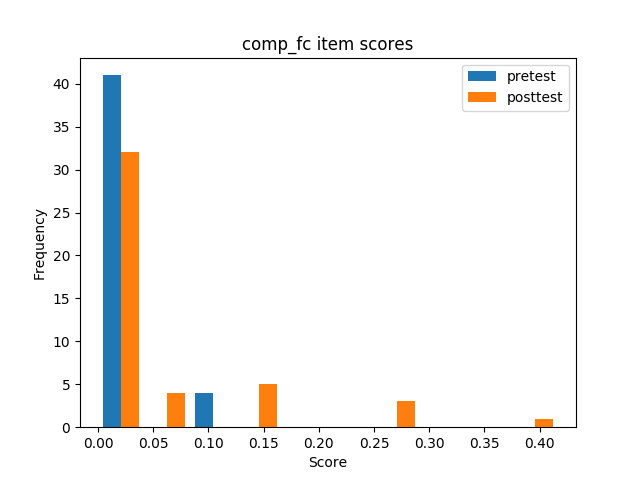
\includegraphics[width=.7\textwidth]{img/comp_fc_diff.png}
    \caption{A histogram depicting the scores on the comprehension section of the pre- and posttest per item by flashcard users}
    \label{fig:comp_fc_diff}
\end{figure}
\begin{figure}
    \centering
    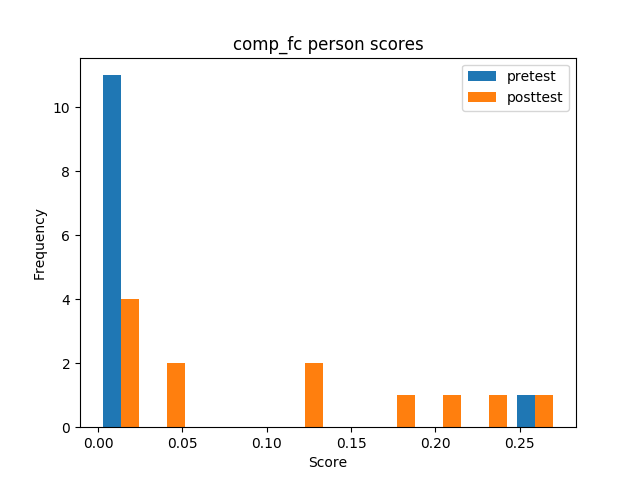
\includegraphics[width=.7\textwidth]{img/comp_fc_abil.png}
    \caption{A histogram depicting the scores on the comprehension section of the pre- and posttest per flashcard user}
    \label{fig:comp_fc_abil}
\end{figure}

\begin{longtable}[c]{@{}lrrrrrrrrrr@{}}
\caption{Flashmap condition}
\endfirsthead
\endhead
\toprule\addlinespace
& N & min & max & mean & var & skew & kurt & norm-t &
norm-p & $\alpha$
\\\addlinespace
\midrule
\textbf{ctt:total} & 22 & 0 & 8 & 1.27 & 3.92 & 2.06 & 4.13 & 22.828 &
0.0000 & 0.7202
\\\addlinespace
\textbf{ctt:pretest} & 11 & 0 & 4 & 0.82 & 1.56 & 1.64 & 1.82 & 12.332 &
0.0021 & 0.5351
\\\addlinespace
\textbf{ctt:posttest} & 11 & 0 & 8 & 1.73 & 6.22 & 1.58 & 1.62 & 11.397
& 0.0034 & 0.7566
\\\addlinespace
\textbf{ctt:abs\_learn\_gain} & 11 & -1 & 4 & 0.91 & 2.89 & 1.04 & -0.35
& 3.526 & 0.1715 & 0.5351
\\\addlinespace
\textbf{ctt:rel\_learn\_gain} & 11 & 0 & 0 & 0.04 & 0.00 & 1.09 & -0.23
& 3.961 & 0.1380 & 0.5351
\\\addlinespace
\textbf{irt:total} & 22 & -1 & 3 & 0.01 & 2.83 & 0.65 & -1.02 & 3.743 &
0.1539 & 0.6260
\\\addlinespace
\textbf{irt:pretest} & 11 & -1 & 3 & -0.00 & 2.98 & 0.91 & -0.34 & 2.786
& 0.2483 & 0.5317
\\\addlinespace
\textbf{irt:posttest} & 11 & -2 & 2 & 0.01 & 3.41 & 0.19 & -1.62 & 4.801
& 0.0907 & 0.6901
\\\addlinespace
\textbf{irt:abs\_learn\_gain} & 11 & -1 & 2 & 0.01 & 1.71 & 1.00 & -0.12
& 3.564 & 0.1683 & 0.5317
\\\addlinespace
\textbf{irt:rel\_learn\_gain} & 11 & 0 & 0 & 0.02 & 0.00 & 0.99 & -0.11
& 3.521 & 0.1720 & 0.5317
\\\addlinespace
\textbf{fixed irt:total} & 22 & -1 & 3 & 0.05 & 2.92 & 0.66 & -1.01 &
3.727 & 0.1551 & 0.6277
\\\addlinespace
\textbf{fixed irt:pretest} & 11 & 0 & 4 & 1.54 & 2.10 & 0.93 & -0.32
& 2.893 & 0.2354 & 0.4888
\\\addlinespace
\textbf{fixed irt:posttest} & 11 & -1 & 3 & 0.57 & 3.81 & 0.15 &
-1.64 & 5.133 & 0.0768 & 0.6957
\\\addlinespace
\textbf{fixed irt:abs\_learn\_gain} & 11 & -2 & 1 & -0.97 & 1.88 &
1.08 & 0.01 & 4.284 & 0.1174 & 0.4888
\\\addlinespace
\textbf{fixed irt:rel\_learn\_gain} & 11 & 0 & 0 & 0.00 & 0.00 & 1.08
& 0.01 & 4.277 & 0.1178 & 0.4888
\\\addlinespace
\bottomrule
    \label{tab:comp_fm}
\end{longtable}

\begin{figure}
    \centering
    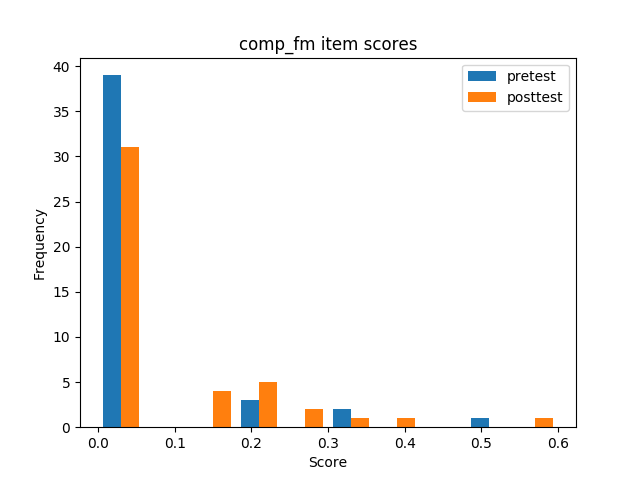
\includegraphics[width=.7\textwidth]{img/comp_fm_diff.png}
    \caption{A histogram depicting the scores on the comprehension section of the pre- and posttest per item by flashmap users}
    \label{fig:comp_fm_diff}
\end{figure}
\begin{figure}
    \centering
    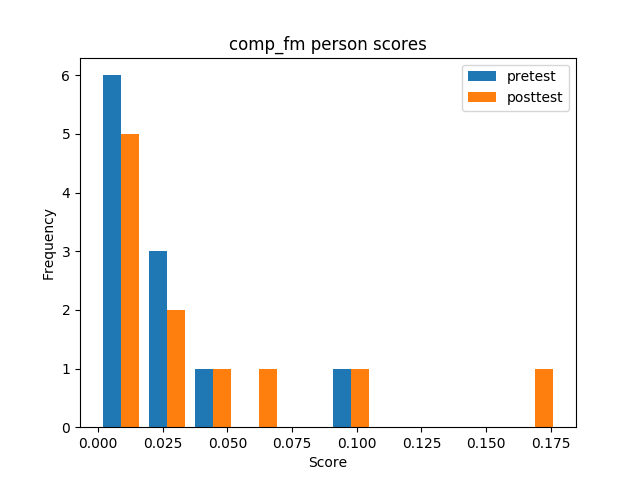
\includegraphics[width=.7\textwidth]{img/comp_fm_abil.png}
    \caption{A histogram depicting the scores on the comprehension section of the pre- and posttest per flashmap user}
    \label{fig:comp_fm_abil}
\end{figure}

\begin{longtable}[c]{@{}lrrrrrrrrrr@{}}
\caption{Combined conditions}
\endfirsthead
\endhead
\toprule\addlinespace
& N & min & max & mean & var & skew & kurt & norm-t &
norm-p & $\alpha$
\\\addlinespace
\midrule
\textbf{ctt:total} & 46 & 0 & 8 & 1.30 & 3.99 & 1.58 & 1.77 & 19.890 &
0.0000 & 0.7140
\\\addlinespace
\textbf{ctt:pretest} & 23 & 0 & 4 & 0.57 & 1.44 & 2.19 & 3.53 & 23.159 &
0.0000 & 0.6350
\\\addlinespace
\textbf{ctt:posttest} & 23 & 0 & 8 & 2.04 & 5.59 & 0.98 & -0.02 & 4.808
& 0.0903 & 0.6951
\\\addlinespace
\textbf{ctt:abs\_learn\_gain} & 23 & -1 & 6 & 1.48 & 4.35 & 0.97 & -0.34
& 4.419 & 0.1097 & 0.6350
\\\addlinespace
\textbf{ctt:rel\_learn\_gain} & 23 & 0 & 0 & 0.05 & 0.00 & 0.95 & -0.42
& 4.277 & 0.1178 & 0.6350
\\\addlinespace
\textbf{irt:total} & 46 & -1 & 3 & 0.00 & 2.33 & 0.81 & -0.90 & 8.324 &
0.0156 & 0.6015
\\\addlinespace
\textbf{irt:pretest} & 23 & -1 & 4 & 0.01 & 2.56 & 1.65 & 1.53 & 13.943
& 0.0009 & 0.4629
\\\addlinespace
\textbf{irt:posttest} & 23 & -1 & 2 & 0.00 & 2.04 & 0.19 & -1.52 &
11.285 & 0.0035 & 0.6781
\\\addlinespace
\textbf{irt:abs\_learn\_gain} & 23 & -3 & 3 & -0.01 & 2.86 & 0.32 &
-0.85 & 1.311 & 0.5192 & 0.4629
\\\addlinespace
\textbf{irt:rel\_learn\_gain} & 23 & 0 & 0 & 0.02 & 0.00 & 0.24 & -0.77
& 0.786 & 0.6749 & 0.4629
\\\addlinespace
\textbf{fixed irt:total} & 46 & -2 & 2 & -0.62 & 2.30 & 0.82 & -0.86
& 8.005 & 0.0183 & 0.6058
\\\addlinespace
\textbf{fixed irt:pretest} & 23 & -1 & 4 & 0.04 & 2.52 & 1.66 & 1.54
& 13.979 & 0.0009 & 0.4618
\\\addlinespace
\textbf{fixed irt:posttest} & 23 & -1 & 2 & -0.23 & 1.97 & 0.17 &
-1.56 & 12.676 & 0.0018 & 0.6732
\\\addlinespace
\textbf{fixed irt:abs\_learn\_gain} & 23 & -3 & 2 & -0.26 & 2.85 &
0.27 & -0.87 & 1.246 & 0.5362 & 0.4618
\\\addlinespace
\textbf{fixed irt:rel\_learn\_gain} & 23 & 0 & 0 & 0.02 & 0.00 & 0.18
& -0.76 & 0.640 & 0.7262 & 0.4618
\\\addlinespace
\bottomrule
    \label{tab:comp_gen}
\end{longtable}

\begin{figure}
    \centering
    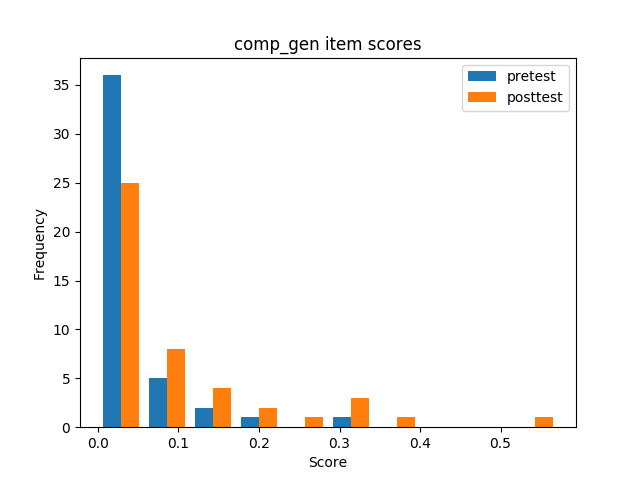
\includegraphics[width=.7\textwidth]{img/comp_gen_diff.png}
    \caption{A histogram depicting the scores on the comprehension section of the pre- and posttest per item by users}
    \label{fig:comp_gen_diff}
\end{figure}
\begin{figure}
    \centering
    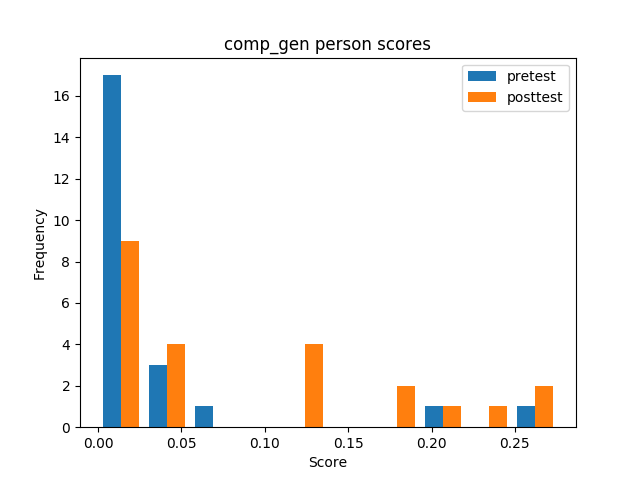
\includegraphics[width=.7\textwidth]{img/comp_gen_abil.png}
    \caption{A histogram depicting the scores on the comprehension section of the pre- and posttest per user}
    \label{fig:comp_gen_abil}
\end{figure}

\section{Comparisons of the comprehension questions}

\subsection{Pre- and posttest comparisons}

\begin{longtable}[c]{@{}lrrrr@{}}
\caption{Flashcard condition}
\endfirsthead
\endhead
\toprule\addlinespace
& \textbf{MW k} & \textbf{MW p} &
\textbf{t-test k} & \textbf{t-test p}
\\\addlinespace
\midrule
\textbf{ctt} & -2.683 & 0.0136 & -2.683 & 0.0162
\\\addlinespace
\textbf{irt} & -0.146 & 0.8852 & -0.146 & 0.8852
\\\addlinespace
\textbf{fixed irt} & 1.856 & 0.0768 & 1.856 & 0.0770
\\\addlinespace
\bottomrule
    \label{tab:comp_pp_fc_comp}
\end{longtable}

\begin{longtable}[c]{@{}lrrrr@{}}
\caption{Flashmap condition}
\endfirsthead
\endhead
\toprule\addlinespace
& \textbf{MW k} & \textbf{MW p} &
\textbf{t-test k} & \textbf{t-test p}
\\\addlinespace
\midrule
\textbf{ctt} & -1.081 & 0.2926 & -1.081 & 0.2971
\\\addlinespace
\textbf{irt} & -0.018 & 0.9854 & -0.018 & 0.9854
\\\addlinespace
\textbf{fixed irt} & 1.318 & 0.2024 & 1.318 & 0.2036
\\\addlinespace
\bottomrule
    \label{tab:comp_pp_fm_comp}
\end{longtable}

\begin{longtable}[c]{@{}lrrrr@{}}
\caption{Combined conditions}
\endfirsthead
\endhead
\toprule\addlinespace
& \textbf{MW k} & \textbf{MW p} &
\textbf{t-test k} & \textbf{t-test p}
\\\addlinespace
\midrule
\textbf{ctt} & -2.674 & 0.0105 & -2.674 & 0.0116
\\\addlinespace
\textbf{irt} & 0.023 & 0.9818 & 0.023 & 0.9818
\\\addlinespace
\textbf{fixed irt} & 0.595 & 0.5549 & 0.595 & 0.5549
\\\addlinespace
\bottomrule
    \label{tab:comp_pp_gen_comp}
\end{longtable}

\FloatBarrier
\subsection{Learning gain comparisons between conditions}

\begin{longtable}[c]{@{}lrrrr@{}}
\caption{Classical test theory}
\endfirsthead
\endhead
\toprule\addlinespace
& \textbf{MW k} & \textbf{MW p} &
\textbf{t-test k} & \textbf{t-test p}
\\\addlinespace
\midrule
\textbf{total} & 0.102 & 0.9195 & 0.102 & 0.9194
\\\addlinespace
\textbf{pretest} & -0.967 & 0.3446 & -0.963 & 0.3466
\\\addlinespace
\textbf{posttest} & 0.605 & 0.5515 & 0.603 & 0.5531
\\\addlinespace
\textbf{abs\_learn\_gain} & 1.270 & 0.2179 & 1.288 & 0.2124
\\\addlinespace
\textbf{rel\_learn\_gain} & 1.197 & 0.2448 & 1.211 & 0.2399
\\\addlinespace
\bottomrule
    \label{tab:comp_cond_ctt_comp}
\end{longtable}

\begin{longtable}[c]{@{}lrrrr@{}}
\caption{Item response theory}
\endfirsthead
\endhead
\toprule\addlinespace
& \textbf{MW k} & \textbf{MW p} &
\textbf{t-test k} & \textbf{t-test p}
\\\addlinespace
\midrule
\textbf{total} & 0.071 & 0.9436 & 0.072 & 0.9430
\\\addlinespace
\textbf{pretest} & -0.132 & 0.8961 & -0.132 & 0.8965
\\\addlinespace
\textbf{posttest} & -0.002 & 0.9982 & -0.002 & 0.9982
\\\addlinespace
\textbf{abs\_learn\_gain} & 0.112 & 0.9116 & 0.115 & 0.9097
\\\addlinespace
\textbf{rel\_learn\_gain} & 0.064 & 0.9496 & 0.066 & 0.9484
\\\addlinespace
\bottomrule
    \label{tab:comp_cond_irt_comp}
\end{longtable}

\begin{longtable}[c]{@{}lrrrr@{}}
\caption{Item response theory with fixed item difficulties}
\endfirsthead
\endhead
\toprule\addlinespace
& \textbf{MW k} & \textbf{MW p} &
\textbf{t-test k} & \textbf{t-test p}
\\\addlinespace
\midrule
\textbf{total} & -2.188 & 0.0340 & -2.202 & 0.0330
\\\addlinespace
\textbf{pretest} & -1.748 & 0.0950 & -1.756 & 0.0936
\\\addlinespace
\textbf{posttest} & -1.849 & 0.0785 & -1.842 & 0.0802
\\\addlinespace
\textbf{abs\_learn\_gain} & -0.407 & 0.6882 & -0.415 & 0.6826
\\\addlinespace
\textbf{rel\_learn\_gain} & -0.455 & 0.6537 & -0.465 & 0.6476
\\\addlinespace
\bottomrule
    \label{tab:comp_cond_adj_irt_comp}
\end{longtable}

\begin{figure}
    \centering
    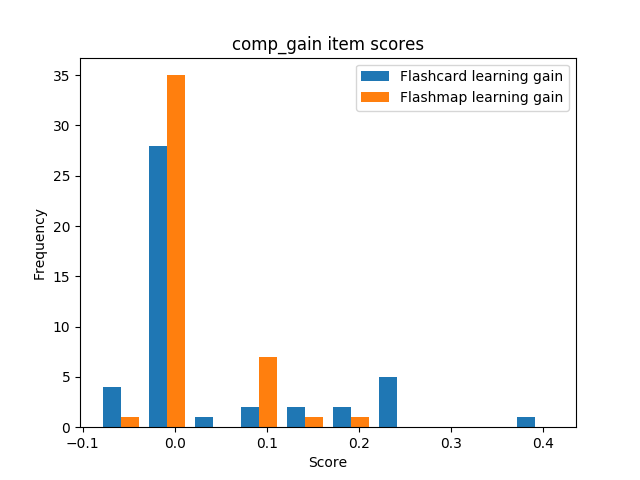
\includegraphics[width=.7\textwidth]{img/comp_gain_diff.png}
    \caption{A comparison of figure~\protect\ref{fig:comp_fc_diff} and~\protect\ref{fig:comp_fm_diff}, with the pretest score subtracted from the posttest score}
    \label{fig:comp_gain_diff}
\end{figure}
